\assignementTitle{Полимеразная цепная реакция с геномной ДНК}{16}{}
\subsection*{Необходимое оборудование и реактивы}
\begin{itemize}
\item ДНК-матрица
\item 2 праймера (форвард и реверс)
\item Мастер-микс (ПЦР буфер, дезоксинуклеозидтрифосфаты (дНТФ или dNTP), полимераза)
\item Стерильная вода
\item Микропробирки 0,2 мл для амплификатора
\item Амплификатор
\item Агарозный гель
\item Буфер с красителем для нанесения проб на гель (4X Gel loading dye)
\item ДНК-маркер
\item Камера и источник питания для проведения электрофореза
\item Трансиллюминатор
\end{itemize}

\subsection*{Протокол процедуры}

\begin{enumerate}
    \item Подготовить реакционные смеси для постановки ПЦР согласно таблице
    
    \begin{tabular}{|p{4cm}|p{2.5cm}|p{2.5cm}|p{3cm}|}
        \hline
        & Контрольная линия & Тестовая 
        
        линия & Отрицательный контроль \\
        \hline
        H2O & 19,5 мкл & 18 мкл & 21 мкл \\
        \hline
        Мастер-микс, X2
        
        (буфер, dNTP, 
        
        полимераза) & 25 мкл & 25 мкл & 25 мкл \\
        \hline
        Праймер F, X25 & 2 мкл & 2 мкл & 2 мкл \\ 
        \hline
        Праймер R, X25 & 2 мкл & 2 мкл & 2 мкл \\ 
        \hline
        ДНК-матрица

        (100-150 нг) & 1,5 мкл (при концентрации ДНК 100нг/мкл) & 3 мкл (при концентрации ДНК 50нг/мкл) & - \\
        \hline
        \hline
        Общий объем = 50 мкл & 50 мкл & 50 мкл & 50 мкл \\ 
        \hline       
    \end{tabular}

    \item На пробирках обязательно указать номер рабочего места!
    \item Перемешать реакционную смесь пипеткой.
    \item Если в реакционной смеси наблюдаются пузырьки воздуха, эти образцы следует центрифугировать.
    \item Настроить программу амплификатора в соответствии с заданными параметрами (выполняет ассистент на площадке):
    
    \begin{tabular}{|c|c|c|c|}
        \hline
        Первичная денатурация ДНК & $95^{\circ}С$ & 3 мин & \\	 
        \hline
        Денатурация ДНК & $95^{\circ}С$ & 30 сек & 	\\
        \cline{1-2}
        Отжиг праймеров & $58^{\circ}С$ & 15 сек & 30 циклов \\
        \cline{1-2}
        Элонгация & $72^{\circ}С$ & 45 сек & \\
        \hline
        Финальная достройка & $72^{\circ}С$ & 5 мин & \\	 
        \hline
        Хранение & $12^{\circ}С$ & $\infty$ & \\
        \hline 
    \end{tabular}

    \item Установить пробирки в амплификатор и запустить программу (выполняет ассистент на площадке).
    \item После окончания ПЦР отобрать 10 мкл каждого образца и добавить \underline{3,3} мкл четырехкратного красителя. Перемешать реакционную смесь до равномерного распределения красителя.
    \item Перенести подготовленные пробы в гель для электрофореза в следующем порядке:  6 мкл маркера длин ДНК фрагментов 1kb, отрицательный контроль, проба с контрольной линии, проба с тестовой линии.
    \item Провести электрофорез в течение 30 мин.
    \item После завершения электрофореза сделать фотографию геля.
    
    \begin{tabular}{cc}
        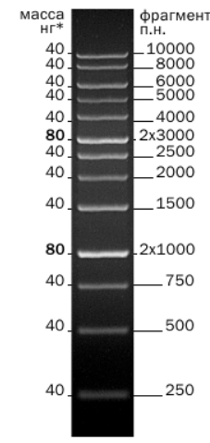
\includegraphics[height=8cm]{1.png}& 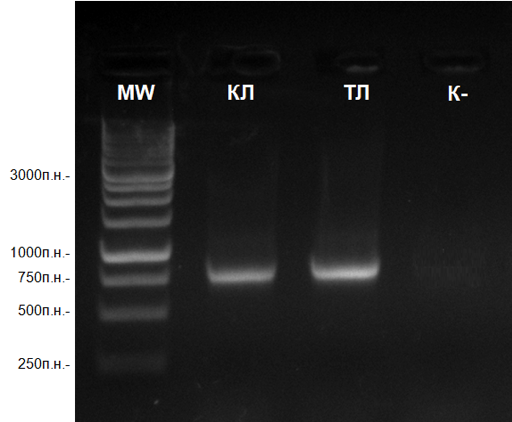
\includegraphics[height=8cm]{2.png}\\
    \end{tabular}

    Слева — расшифровка полос маркера длин ДНК фрагментов, справа — фотография электрофореза для продуктов ПЦР: КЛ — продукт, полученный при амплификации с ДНК контрольной линии, ТЛ — ампликон для тестовой линии, К- — отрицательный контроль. Размер ампликонов примерно соответствует 750 п.н.

    \item По результатам электрофореза оценить размер ампликона и сопоставить результат с данными, полученными в результате дизайна ПЦР in silico.

    Длина ампликона по результатам фореза: 750 п.н.

    Предсказанная длина ампликона: 761 п.н.

\end{enumerate}

\markSection

\begin{tabular}{|p{11cm}|p{3cm}|}
    \hline
    \textbf{Описание критерия} & \textbf{Балл} \\
    \hline
    Расчет состава р.с.: 

    4б — все вычисления сделаны правильно, 

    2б — ошибка в расчете для одной из проб, 

    0б — состав 2 и более проб рассчитан неверно & 4 \\
    \hline
    Объем р.с. после приготовления для всех проб = 50 мкл: 2 или 0 & 2 \\
    \hline
    Расчет объема 4Х красителя: 2 или 0

    (допускается округление до целых мкл) & 2 \\
    \hline
    Соблюден порядок нанесения образцов на гель 

    (MW, К-, контр.л., тест.л.): 1 или 0 & 1 \\
    \hline
    В К- отсутствует продукт: 1 или 0 & 1 \\
    Контрольная линия: 
    яркость полосы продукта соответствует наиболее интенсивным полосам маркера — 2б, 
    яркость меньше — 1б, 
    продукт не визуализируется или не той длины — 0	2
    Тестовая линия: яркость полосы продукта соответствует наиболее интенсивным полосам маркера — 2б, 
    яркость меньше — 1б, 
    продукт не визуализируется или не той длины — 0 & 2 \\
    \hline
    Длина ампликона по фотографии фореза определена верно: 2 или 0 & 2 \\
    \hline
    Команде потребовалась помощь в работе с протоколом & (- 2) \\
    \hline
    Команда не уложилась в регламент & (- 2) \\
    \hline
    \hline
    \textbf{Итог} & \textbf{16} \\
    \hline 
\end{tabular}